\chapter{\cite{蒋宗礼2013}(第4章 正则表达式)}

\emph{主要内容}
\begin{itemize}
	\item 典型$RE$的构造。
	\item 与$RE$等价$FA$的构造方法。
	\item 与$DFA$等价的$RE$的构造。
	\item 重点
		\subitem{-} $RE$的概念。
		\subitem{-} $RE$与$DFA$的等价性。
	\item 难点
	    \subitem{-} $RE$与$DFA$的等价性证明。 
\end{itemize}

\section{RE的形式定义}
\begin{definition}\label{RE_Def} 正则表达式(regular expression,RE)\\
	设$\Sigma$是一个字母表,以递归形式定义正则表达式:
	\begin{enumerate}
		\item $\emptyset$是$\Sigma$上的$RE$,它表示语言$\emptyset$;
		\item $\epsilon$是$\Sigma$上的$RE$,它表示语言$\{\epsilon\}$;
		\item 对于$\forall a\in\Sigma,a$是$\Sigma$上的$RE$,它便是语言$\{a\}$.
		\item 如果$r,s$分别是$\Sigma$上表示语言$R,S$的$RE$,则:
			\subitem $r,s$的“和”$(r+s)$是$\Sigma$上的$RE,(r+s)$表达的语言为$R\cup S$;
			\subitem $r,s$的“乘积”$(rs)$是$\Sigma$上的$RE,(rs)$表达的语言为$RS$;
			\subitem $r$的克林闭包$(r^\ast)$是$\Sigma$上的$RE,(r^\ast)$表达的语言为$R^\ast$;
		\item 只有满足1,2,3,4的才是$\Sigma$上的$RE$.
	\end{enumerate}
\end{definition}

\begin{example} 设$\Sigma=\{0,1\}$
	\begin{itemize}
		\item $0$,表示语言$\{0\}$
		\item $1$,表示语言$\{1\}$
		\item $(0+1)$,表示语言$\{0,1\}$
		\item $(01)$,表示语言$\{01\}$
		\item $(0+1)^\ast$,表示语言$\{0,1\}^\ast$
		\item $(00)(00)^\ast$,表示语言$\{00\}\{00\}^\ast$
		\item $(0+1)^\ast(0+1)(0+1)^\ast$,表示语言$\{0,1\}^+$
		\item $(0+1)^\ast000(0+1)^\ast$,表示$\{0,1\}$上的至少含有3个连续$0$的串组成的语言
		\item $(0+1)^\ast01$,表示所有以$01$结尾的$0,1$字符串组成的语言
		\item $1(0+1)^\ast0$,表示所有以$1$开头,并且以$0$结尾的$0,1$字符串组成的语言
	\end{itemize}
\end{example}

\emph{约定}
\begin{enumerate}
	\item $r$的正闭包$r^+$表示$r$与$(r^\ast)$的乘积以及$(r^\ast)$与$r$的乘积:
	\[r^+ = rr^\ast = r^\ast r\]
	\item 闭包运算的优先级最高,乘运算的优先级次之,加运算$"+"$的优先级最低。
	\item 在意义明确时,$RE\quad r$表示的语言记为$L(r)$,也可以直接地记为$r$。
	\item 加、乘、闭包运算均执行左结合规则。	
\end{enumerate}

\begin{definition}
	设$r,s$是字母表$\Sigma$上的正则表达式,如果$L(r)=L(s)$,则称$r$和$s$\emph{相等(equivalence,也称为等价)}。
\end{definition}

几个基本结论
\begin{enumerate}
	\item 结合律:
		\subitem $(rs)t=r(st)$
		\subitem $(r+s)+t=r+(s+t)$
	\item 分配律:
		\subitem $r(s+t)=rs+rt$
		\subitem $(s+t)r=sr+tr$
	\item 交换律:$r+s=s+r$
	\item 幂等律:$r+r=r$
	\item 加法运算零元素:$r+\emptyset=r$
	\item 乘法运算单位元:$r\epsilon=\epsilon r=r$
	\item 乘法运算零元素:$r\emptyset=\emptyset r=\emptyset$
	\item $L(\emptyset)=\emptyset$
	\item $L(\epsilon)=\{\epsilon\}$
	\item $L(a)=\{a\}, a\in \Sigma$
	\item $L(rs)=L(r)L(s)$
	\item $L(r+s)=L(r)\cup L(s)$
	\item $L(r^\ast)=(L(r))^\ast$
	\item $L(\emptyset^\ast)=\{\epsilon\}$
	\item $L((r+\epsilon)^\ast)=L(r^\ast)$
	\item $L((r^\ast)^\ast)=L(r^\ast)$
	\item $L((r^\ast s^\ast)^\ast)=L((r+s)^\ast)$
	\item 如果$L(r)\subseteq L(s)$,则$r+s=s$
	\item $L(r^n)=(L(r))^n$
	\item $r^n r^m = r^{n+m}$
\end{enumerate}

\begin{definition}
	设$r$是字母表$\Sigma$上的一个正则表达式,$r$的$n$次幂定义为:
	\begin{enumerate}
		\item $r^0=\epsilon$
		\item $r^n=r^{n-1}r,(n\ge 1)$
	\end{enumerate}
\end{definition}

\begin{note}
	一般地,$r+\epsilon\ne r, (rs)^n \ne r^ns^n, rs\ne sr$.
\end{note}

\begin{example} 设$\Sigma = \{0,1\}$\\
	$00$表示语言$\{00\}$;\\
	$(0+1)^\ast 00(0+1)^\ast$表示所有的至少含两个连续$0$的$0,1$串组成的语言;\\
	$(0+1)^\ast 1(0+1)^9$表示所有的倒数第10个字符为$1$的串组成的语言;\\
	$L((0+1)^\ast 011)=\{x|x\text{是以$011$结尾的$0,1
		$串}\}$;\\
	$L(0^+ 1^+ 2^+)=\{0^n 1^m 2^k|m,n,k\ge 1\}$;\\
	$L(0^\ast 1^\ast 2^\ast)=\{0^n 1^m 2^k|m,n,k\ge 0\}$;\\
	$L(1(0+1)^\ast 1+0(0+1)^\ast 0))=\{x|\text{$x$的开头字符与尾字符相同}\}$。
\end{example}

\section{正则表达式RE与FA等价}
\begin{definition}
	正则表达式$r$称为与$FA\quad M$等价,如果$L(r)=L(M)$。
\end{definition}

从开始状态出发,根据状态之间按照转移所确定的后继关系,依次计算出所给$FA$的各个状态$q$对应的$set(q)$,并且最终得到相应的$FA$接受的语言的$RE$表示。 
寻找一种比较“机械”的方法,使得计算机系统能够自动完成$FA$与$RE$之间的转换。 

\begin{figure}[htbp]
	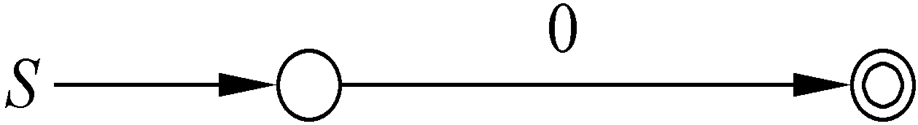
\includegraphics[scale=.4]{0FA}
	\caption{$0$对应的$FA$}
	\label{fig:0FA}       % Give a unique label
\end{figure}

\begin{figure}[htbp]
	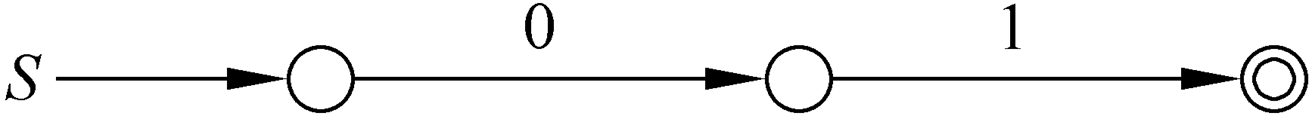
\includegraphics[scale=.4]{01FA}
	\caption{$01$对应的$FA$}
	\label{fig:01FA}       % Give a unique label
\end{figure}

\begin{figure}[htbp]
	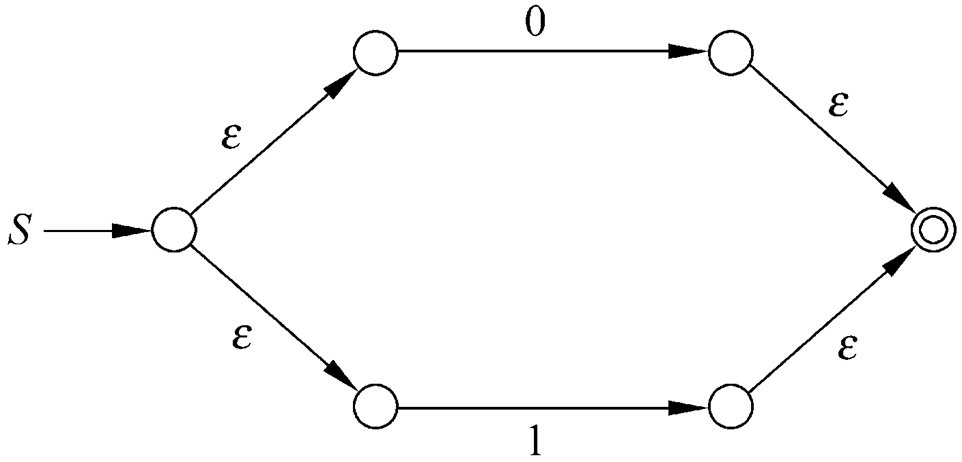
\includegraphics[scale=.4]{0plus1FA}
	\caption{$0+1$对应的$FA$}
	\label{fig:0plus1FA}       % Give a unique label
\end{figure}

\begin{figure}[htbp]
	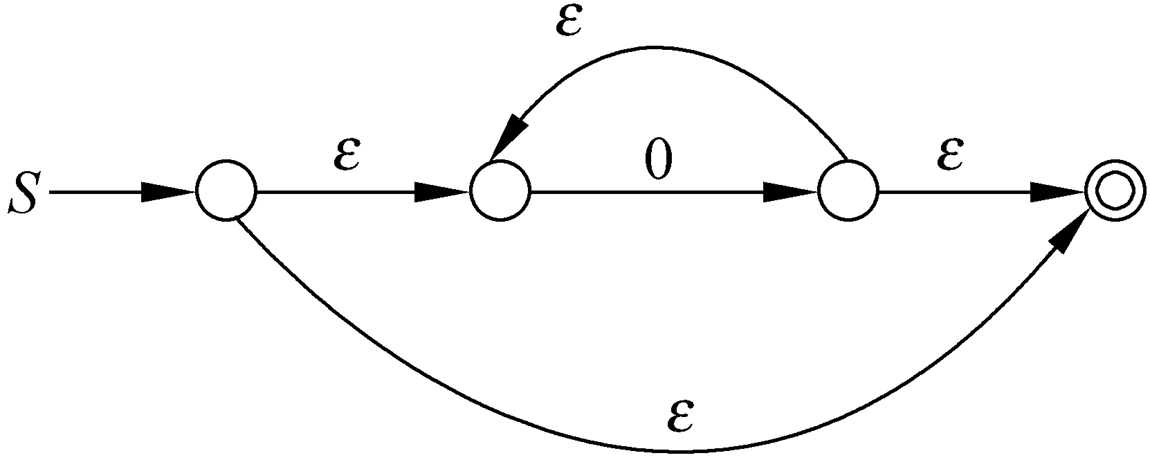
\includegraphics[scale=.4]{0starFA}
	\caption{$0^\ast$对应的$FA$}
	\label{fig:0starFA}       % Give a unique label
\end{figure}

\begin{theorem}
	正则表达式$RE$表示的语言是正则语言$RL$。
\end{theorem}

\begin{proof}
	根据递归表达式的递归定义(\ref{RE_Def}), 施归纳于正则表达式中所含的运算符的个数$n$,证明对于字母表$\Sigma$上的任意正则表达式$r$,存在$FA\quad M$,使得$L(M) = L(r)$ 。
	\begin{itemize}
		\item $M$恰有一个终止状态。
		\item $M$在终止状态下不做移动。
	\end{itemize}

	当$n=0$时,即$r$中不含运算符时,有以下3种情况:
	\begin{enumerate}
		\item $r=\epsilon$,此时图\ref{fig:epsilon_empty_a}(a)所示的$\epsilon -NFA$满足要求。
		\item $r=\emptyset$,此时图\ref{fig:epsilon_empty_a}(b)所示的$\epsilon -NFA$满足要求。
		\item $\forall a\in\Sigma$,此时图\ref{fig:epsilon_empty_a}(c)所示的$\epsilon -NFA$满足要求。
	\end{enumerate}

	所以,结论对$n=0$时成立。
	\begin{figure}[htbp]
		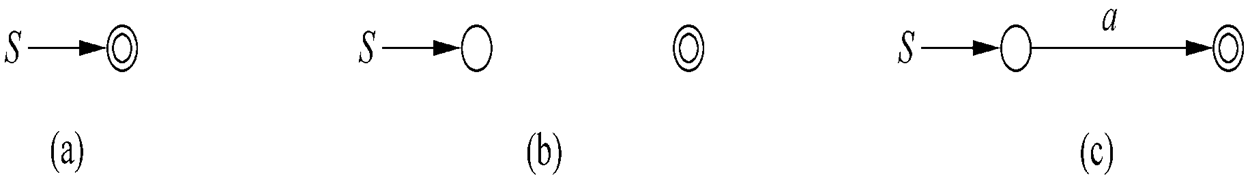
\includegraphics[scale=.45]{epsilon_empty_a}
		\caption{$r=\epsilon,r=\emptyset,r=a$对应的$\epsilon -NFA$}
		\label{fig:epsilon_empty_a}       % Give a unique label
	\end{figure}
    
    假设结论对$n\le k\quad (k\ge 0)$成立,此时有如下$FA$:
    
    $M_1=(Q_1,\Sigma,\delta_1,q_{01},\{f_1\})$
    
    $M_2=(Q_2,\Sigma,\delta_2,q_{02},\{f_2\})$
    
    $L(M_1)=L(r_1), L(M_2)=L(r_2)$
    
    $Q_1\cap Q_2=\emptyset$
    
    \hfill
    
    当$n=k+1$时, $r$有以下3种运算:
    
    \begin{enumerate}
    	\item $r=r_1+r_2$
	    
	    取$q_0,f\notin Q_1\cup Q_2$,令
	    
	    $M=(Q_1\cup Q_2\cup \{q_0,f\},\Sigma,\delta,q_{0},\{f\})$
	    
	    \begin{enumerate}
	    	\item $\delta(q_0,\epsilon)=\{q_{01},q_{02}\}$
	    	\item 对$\forall q\in Q_1,a\in\Sigma\cup\{\epsilon\},\delta(q,a)=\delta_1(q,a)$;\\
	    	对$\forall q\in Q_2,a\in\Sigma\cup\{\epsilon\},\delta(q,a)=\delta_2(q,a)$;
	    	\item $\delta(f_1,\epsilon)=\{f\}$
	    	\item $\delta(f_2,\epsilon)=\{f\}$
	    \end{enumerate}
	    
	    这里构造的$M$,如图(\ref{fig:r_eq_r1_plus_r2})
	    \begin{figure}[htbp]
	    	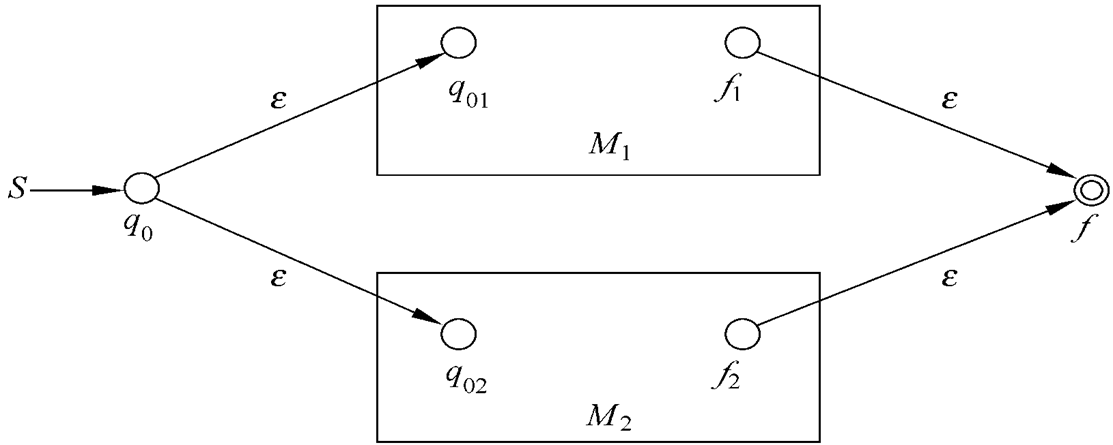
\includegraphics[scale=.45]{r_eq_r1_plus_r2}
	    	\caption{与$r_1+r_2$等价的满足要求的$\epsilon -NFA$}
	    	\label{fig:r_eq_r1_plus_r2}       % Give a unique label
	    \end{figure}
    
        \item $r=r_1r_2$
        
         $M=(Q_1\cup Q_2,\Sigma,\delta,q_{01},\{f_2\})$
        
        \begin{enumerate}
        	\item 对$\forall q\in Q_1-\{f_1\},a\in\Sigma\cup\{\epsilon\},\delta(q,a)=\delta_1(q,a)$;
        	\item 对$\forall q\in Q_2-\{f_2\},a\in\Sigma\cup\{\epsilon\},\delta(q,a)=\delta_2(q,a)$;
        	\item $\delta(f_1,\epsilon)=\{q_{02}\}$
        \end{enumerate}
        
        这里构造的$M$,如图(\ref{fig:r_eq_r1r2})
        \begin{figure}[htbp]
        	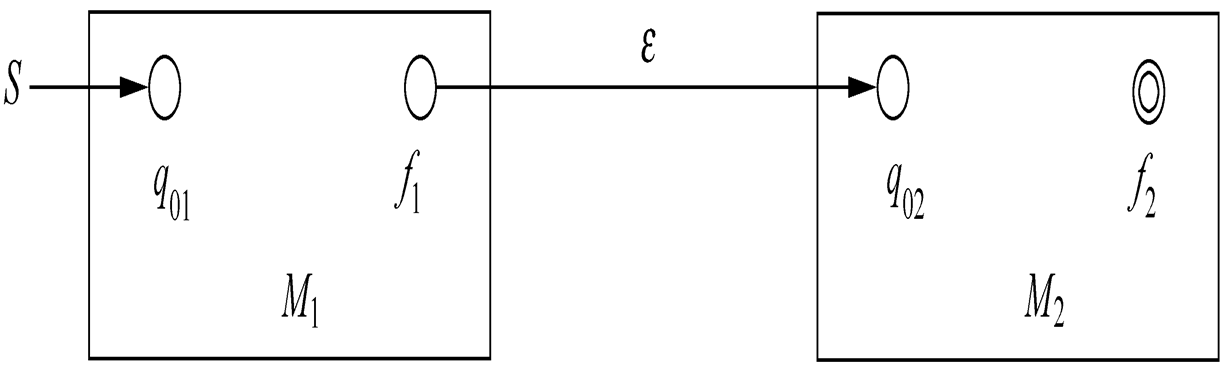
\includegraphics[scale=.45]{r_eq_r1r2}
        	\caption{与$r_1r_2$等价的满足要求的$\epsilon -NFA$}
        	\label{fig:r_eq_r1r2}       % Give a unique label
        \end{figure}
    
	    \item $r=r_1^\ast$
	    
	    $M=(Q_1\cup \{q_0,f\},\Sigma,\delta,q_{0},\{f\})$
	    
	    其中$q_0,f\notin Q_1$, 定义$\delta$为
	    \begin{enumerate}
	    	\item 对$\forall q\in Q_1-\{f_1\},a\in\Sigma,\delta(q,a)=\delta_1(q,a)$;
	    	\item $\delta(f_1,\epsilon)=\{q_{01},f\}$
	    	\item $\delta(q_0,\epsilon)=\{q_{01},f\}$
	    \end{enumerate}
	    
	    这里构造的$M$,如图(\ref{fig:r_eq_r1star})
	    \begin{figure}[htbp]
	    	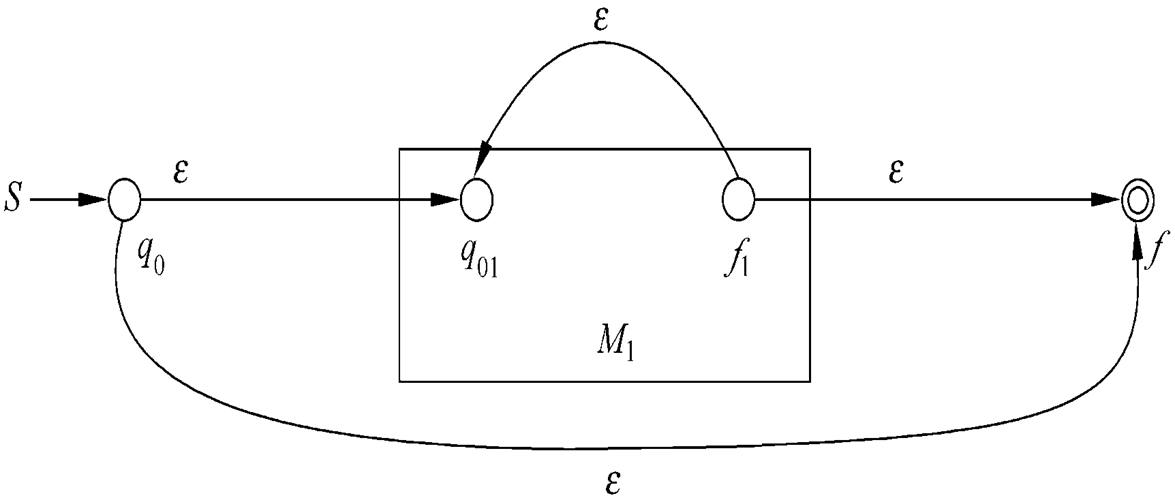
\includegraphics[scale=.45]{r_eq_r1star}
	    	\caption{与$r_1^\ast$等价的满足要求的$\epsilon -NFA$}
	    	\label{fig:r_eq_r1star}       % Give a unique label
	    \end{figure}
	\end{enumerate} 

	因此结论对$n=k+1$成立。由归纳法原理,结论对$\Sigma$上的任意正则表达式成立。
	\hfill$\square$
\end{proof}

\begin{example}
	构造与$(0+1)^\ast 0+(00)^\ast$等价的$FA$。如下图(\ref{fig:ex4-3FA})。  
	\begin{figure}[htbp]
		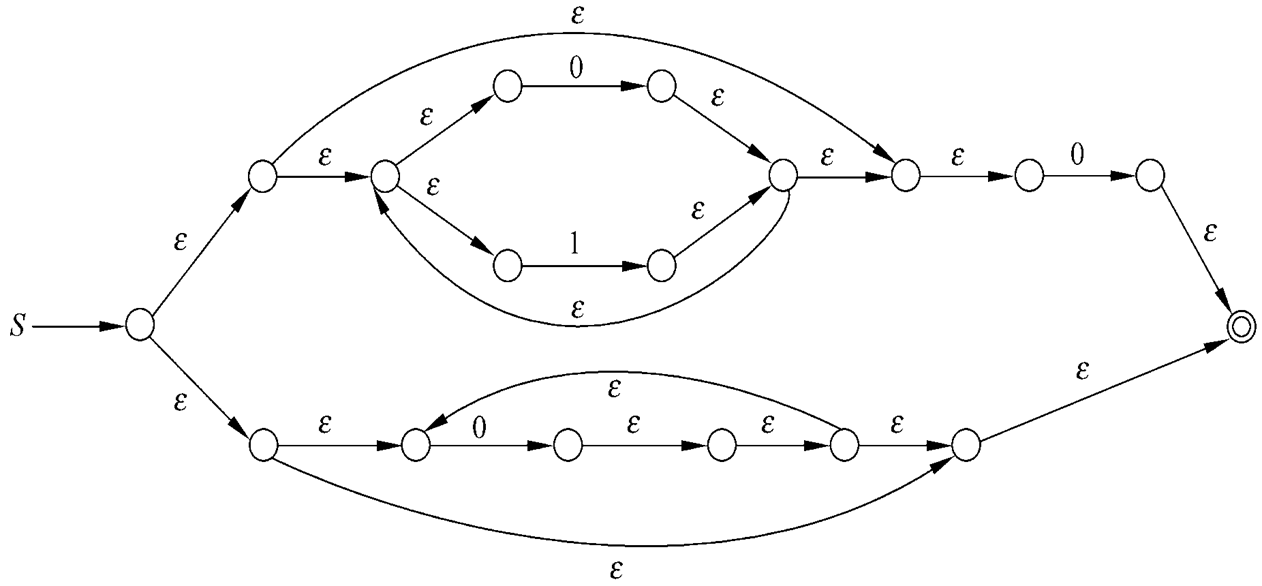
\includegraphics[scale=.45]{ex4-3FA}
		\caption{与$(0+1)^\ast 0+(00)^\ast$等价的$FA$}
		\label{fig:ex4-3FA}       % Give a unique label
	\end{figure}

	按照对$(0+1)^\ast 0+(00)^\ast$的"理解","直接地"构造出的$FA$。
	
	因为,如果$L(r)\subseteq L(s)$,则$r+s=s$, 这里$s=(0+1)^\ast 0,r=(00)^\ast$,因此直接构造出的$FA$如下图(\ref{fig:ex4-3FA1})。 
	\begin{figure}[htbp]
		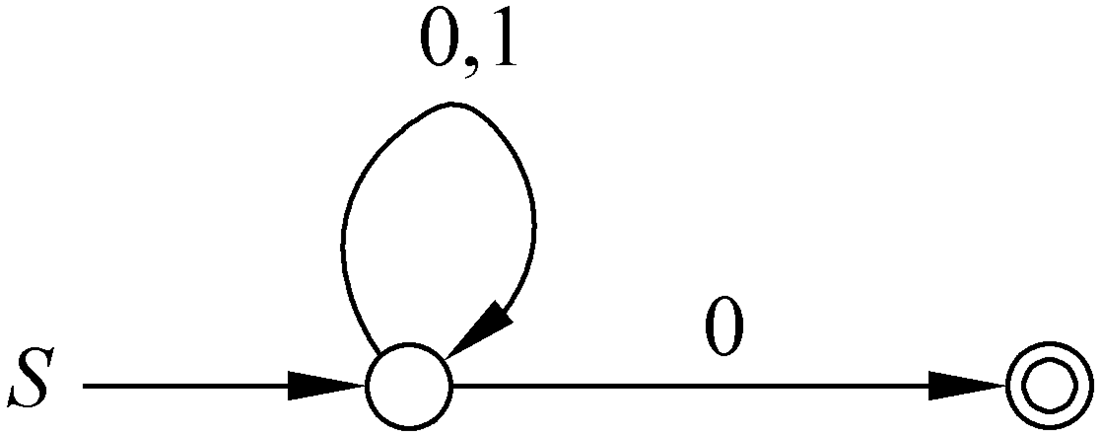
\includegraphics[scale=.45]{ex4-3FA1}
		\caption{与$(0+1)^\ast 0+(00)^\ast$等价的$FA$}
		\label{fig:ex4-3FA1}       % Give a unique label
	\end{figure}
\end{example}

\section{正则语言RL可以用正则表达式RE表示}

\begin{theorem}
	正则语言$RL$可以用正则表达式$RE$表示。
\end{theorem}

设$DFA$
\[M=(\{q_1,q_2,\cdots,q_n\},\Sigma,\delta,q_1,F)\]

令
\[R_{ij}^k = \{x|\delta(q_i,x)=q_j,\text{而且对于$x$的任意前缀$y(y\ne x,y\ne\epsilon)$,如果$\delta(q_i,y)=q_l$,则$l\le k$}\}\]

$R_{ij}^k$表示所有那些将$DFA$从给定状态$q_i$引导到状态$q_j$,并且“途中”不经过(进入并离开)下标大于$k$的状态的所有字符串。值得提醒的是,$i$和$j$的值不受小于等于$k$的限制。

对于$\forall q_i,q_j\in\{q_1,q_2,\cdots,q_n\}, R_{ij}^k$是所有可以将$DFA$从状态$q_i$引导到状态$q_j$的字符串组成的集合。为了便于计算,可以将$R_{ij}^k$递归地定义为:

\[R_{ij}^0 =\begin{cases}
\{a|\delta(q_i,a)=q_j\} &\qquad \text{如果$i\ne j$}\\
\{a|\delta(q_i,a)=q_j\}\cup\{\epsilon\} &\qquad \text{如果$i=j$}
\end{cases}
 \]
 
\[R_{ij}^k = R_{ik}^{k-1}(R_{kk}^{k-1})^\ast R_{kj}^{k-1}\cup R_{ij}^{k-1}\]

显然,
$$L(M)=\bigcup_{q_f\in F}R_{1f}^n$$

当$R_{ij}^0 =\emptyset$时,它对应的正则表达式为$\emptyset$; 当$R_{ij}^0 =\{a_1,a_2,\cdots,a_n\}\ne\emptyset$时,它对应的正则表达式为$a_1+a_2+\cdots+a_n$.

仅当$i=j$时,集合$R_{ij}^0$中含有一个$\epsilon$,而$R_{ij}^k$的表达式中含的都是定义正则表达式时用的运算,所以,容易得到$R_{ij}^k$的正则表达式。

\begin{figure}[htbp]
	\centering
	\begin{minipage}[htbp]{0.3\textwidth}	
	\centerline{} %插入一行,使左右对齐
	\centerline{}
	\begin{tikzpicture}[>=latex, shorten >=1pt,node distance=0.75in, on grid, auto]
	% Vertices of automaton
	%\node[state, initial, accepting] (qi) {$q_i$};
	\node[state] (qi) {$q_i$};
	\node[state](qj) [right=of qi] {$q_j$};
	% Edges of automaton
	\path[->] 
	(qi) edge node {a} (qj);
	\end{tikzpicture}
	\centerline{(a) $R_{ij}^0, i\ne j$}
    \end{minipage}
    \begin{minipage}[htbp]{0.3\textwidth}
	\begin{tikzpicture}[>=latex, shorten >=1pt,node distance=0.75in, on grid, auto]
	% Vertices of automaton
	%\node[state, initial, accepting] (qi) {$q_i$};
	\node[state] (qi) {$q_i$};
	\node[state](qj) [right=of qi] {$q_j$};
	% Edges of automaton
	\path[->] 
	(qi) edge [bend left] node {a} (qj)
	(qi) edge [bend right] node [swap] {$\epsilon$} (qj); 
	\end{tikzpicture}
	\centerline{(b) $R_{ij}^0, i = j$}
    \end{minipage}
    \caption{$R_{ij}^0$对应的$FA$}
    \label{fig:R0-2}       % Give a unique label
\end{figure}

\begin{figure}[htbp]
	\centering
	\begin{tikzpicture}[>=latex, shorten >=1pt,node distance=0.75in, on grid, auto]
	% Vertices of automaton
	%\node[state, initial, accepting] (qi) {$q_i$};
	\node[state] (qi) {$q_i$};
	\node[state](qk) [right=of qi] {$q_k$};
	\node[state](qj) [right=of qk] {$q_j$};
	
	% Edges of automaton
	\path[->] 
	(qi) edge node {$R_{ik}^{k-1}$} (qk)
	(qk) edge node {$R_{kj}^{k-1}$} (qj)
	(qk) edge [loop above] node {$R_{kk}^{k-1}$} (qk)
	%(qi) edge [bend right] node {$R_{kj}^{k-1}$} (qj); %弧标记在上
	(qi) edge [bend right] node [swap] {$R_{ij}^{k-1}$} (qj); %弧标记在下
	\end{tikzpicture}
	\caption{$R_{ij}^k$对应的$FA$}
	\label{fig:Rk}       % Give a unique label
\end{figure}


\paragraph{\textbf{图上作业法}}

典型等价变换示例,见图(\ref{fig:figWork})。

\begin{figure}[htbp]
	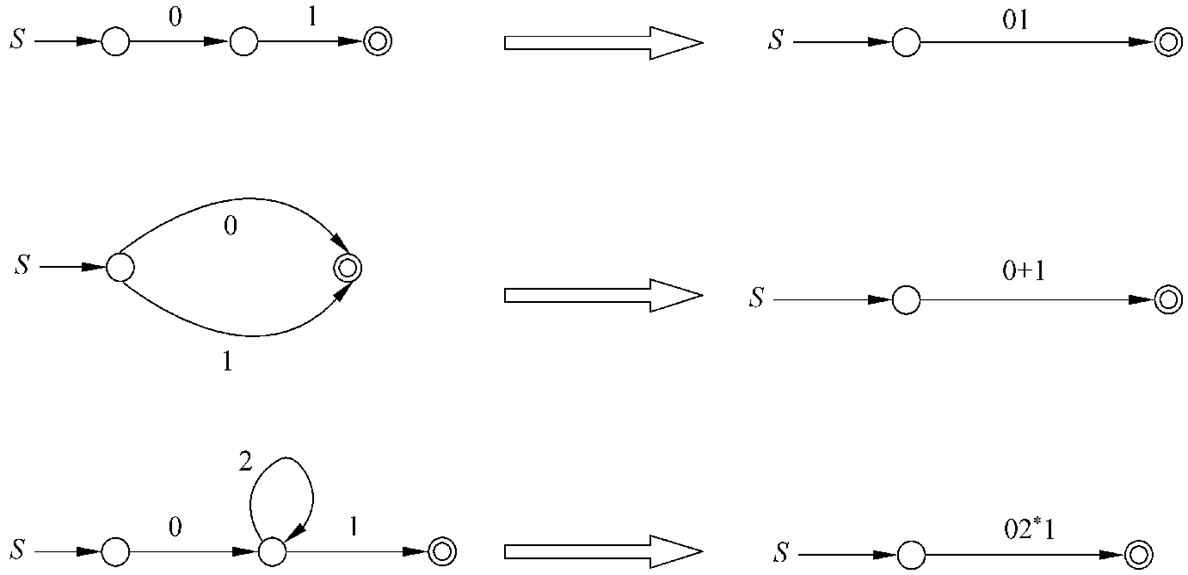
\includegraphics[scale=.45]{figWork}
	\caption{典型等价变换示例}
	\label{fig:figWork}       % Give a unique label
\end{figure}

图上作业法操作步骤
\begin{enumerate}
	\item 预处理:
		\begin{enumerate}
			\item 用标记为$X$和$Y$的状态将$M$“括起来”:
		    \subitem{-} 在状态转移图中增加标记为$X$和$Y$的状态,从标记为$X$的状态到标记为$q_0$的状态引一条标记为$\epsilon$的弧;从标记为$q(q\in F)$的状态到标记为$Y$的状态分别引一条标记为$\epsilon$的弧。
			\item 去掉所有的不可达状态。
		\end{enumerate}
	\item 对通过步骤(1)处理所得到的状态转移图重复如下操作,直到该图中不再包含除了标记为$X$和$Y$外的其他状态,并且这两个状态之间最多只有一条弧。 
		\begin{enumerate}
			\item 并弧
			\subitem{-} 将从$q$到$p$的标记为$r_1,r2,\cdots,r_g$并行弧用从$q$到$p$的、标记为$r_1+r2+\cdots+r_g$的弧取代这$g$个并行弧。 
			\item 去状态1
			\subitem{-} 如果从$q$到$p$有一条标记为$r_1$的弧,从$p$到$t$有一条标记为$r_2$的弧,不存在从状态$p$到状态$p$的弧,将状态$p$和与之关联的这两条弧去掉,用一条从$q$到$t$的标记为$r_1r_2$的弧代替。 
			\item 去状态2
			\subitem{-} 如果从$q$到$p$有一条标记为$r_1$的弧,从$p$到$t$有一条标记为$r_2$的弧,从状态$p$到状态$p$的标记为$r_3$的弧,将状态$p$和与之关联的这三条弧去掉,用一条从$q$到$t$的标记为$r_1r_3^\ast r_2$的弧代替。 
			\item 去状态3
			\subitem{-} 如果图中只有三个状态,而且不存在从标记为$X$的状态到达标记为$Y$的状态的路,则将除标记为$X$的状态和标记为$Y$的状态之外的第3个状态及其相关的弧全部删除。 	
		\end{enumerate}	
	\item 从标记为$X$的状态到标记为$Y$的状态的弧的标记为所求的正则表达式。如果此弧不存在,则所求的正则表达式为$\emptyset$。 	
\end{enumerate}

\begin{example}
	求图(\ref{fig:ex4-4})所示的$DFA$等价的$RE$。
	\begin{figure}[htbp]
		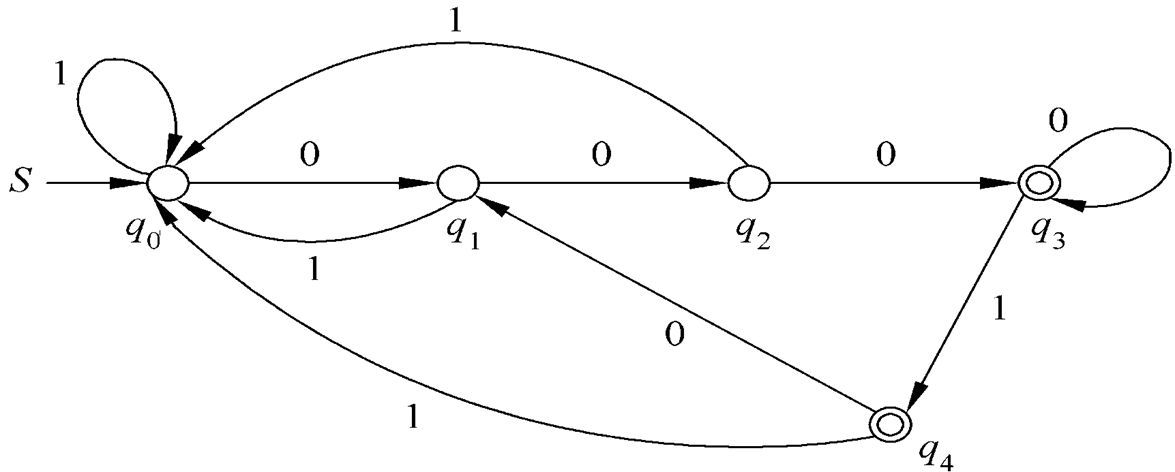
\includegraphics[scale=.45]{ex4-4}
		\caption{由$DFA$构造等价正则表达式的示例$DFA$}
		\label{fig:ex4-4}       % Give a unique label
	\end{figure}
    
    \begin{enumerate}
    	\item 预处理,得到图\ref{fig:ex4-4-1}。
	    \begin{figure}[htbp]
	    	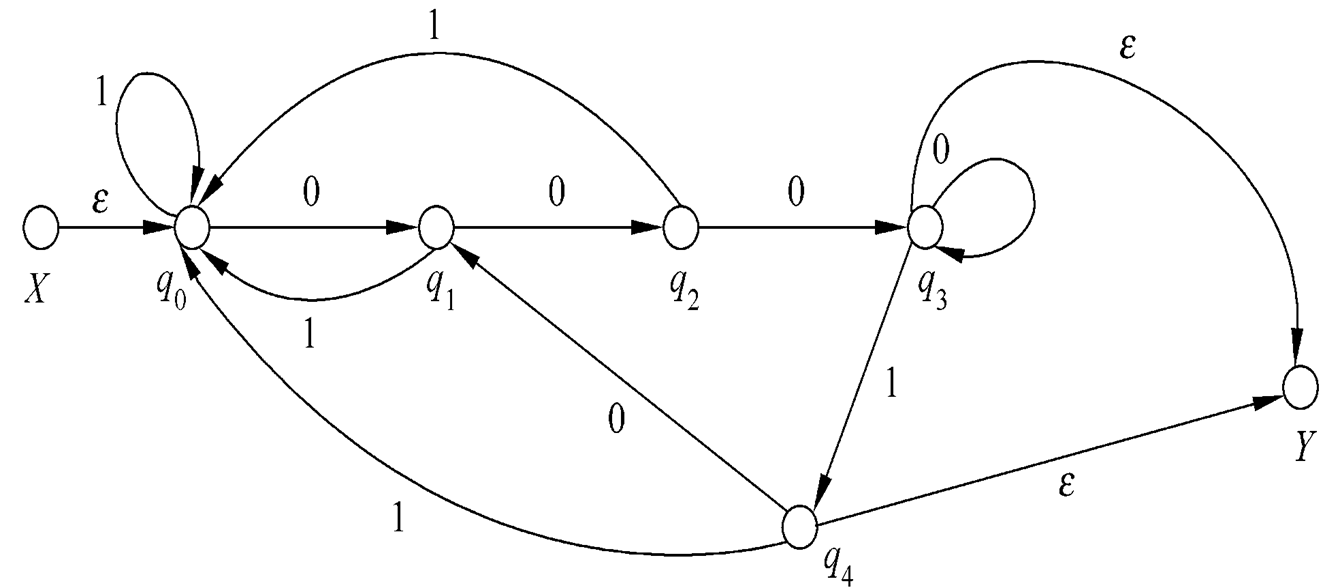
\includegraphics[scale=.45]{ex4-4-1}
	    	\caption{执行步骤(1)后的$DFA$}
	    	\label{fig:ex4-4-1}       % Give a unique label
	    \end{figure}
		\item 去掉状态$q_3$,得到图\ref{fig:ex4-4-2}
		\begin{figure}[htbp]
			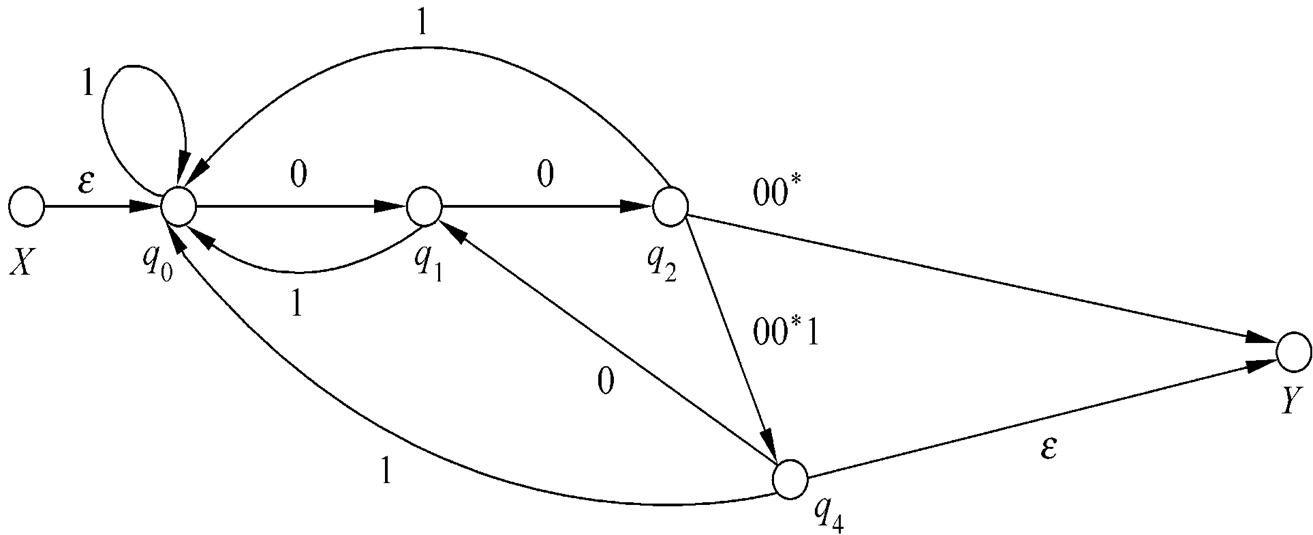
\includegraphics[scale=.45]{ex4-4-2}。
			\caption{去掉状态$q_3$后的$DFA$}
			\label{fig:ex4-4-2}       % Give a unique label
		\end{figure}
	    \item 去掉状态$q_4$,得到图\ref{fig:ex4-4-3}
		\begin{figure}[htbp]
			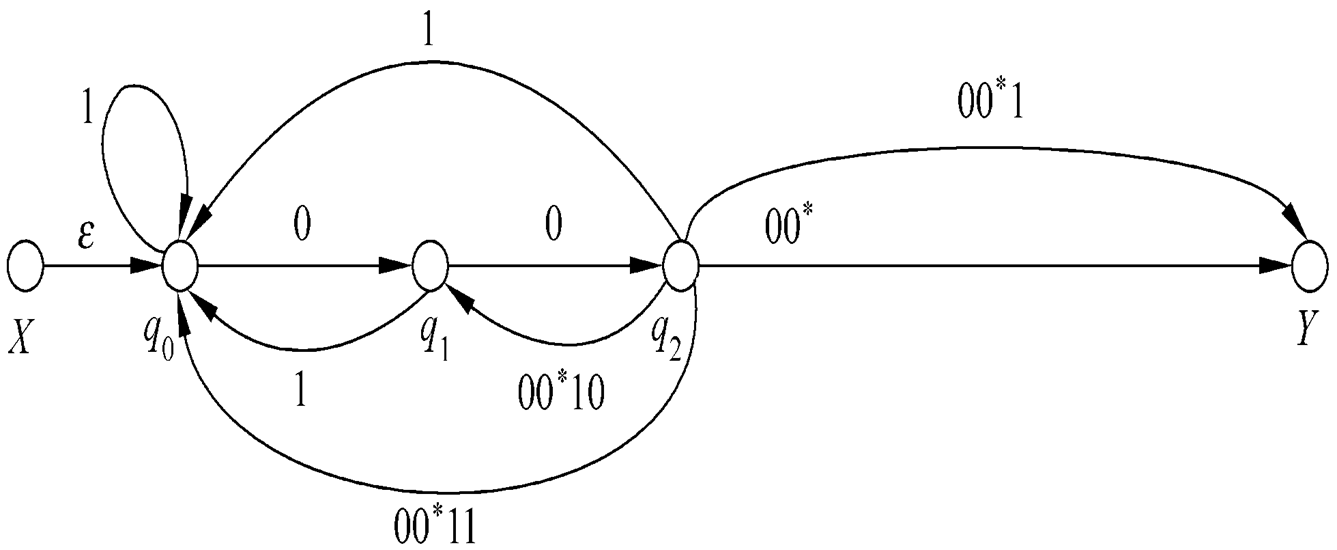
\includegraphics[scale=.45]{ex4-4-3}
			\caption{去掉状态$q_4$后的$DFA$}
			\label{fig:ex4-4-3}       % Give a unique label
		\end{figure}
	    \item 合并从标记为$q_2$的状态到标记为$Y$的状态的两条并行弧。得到图\ref{fig:ex4-4-4}。 
	    \begin{figure}[htbp]
	    	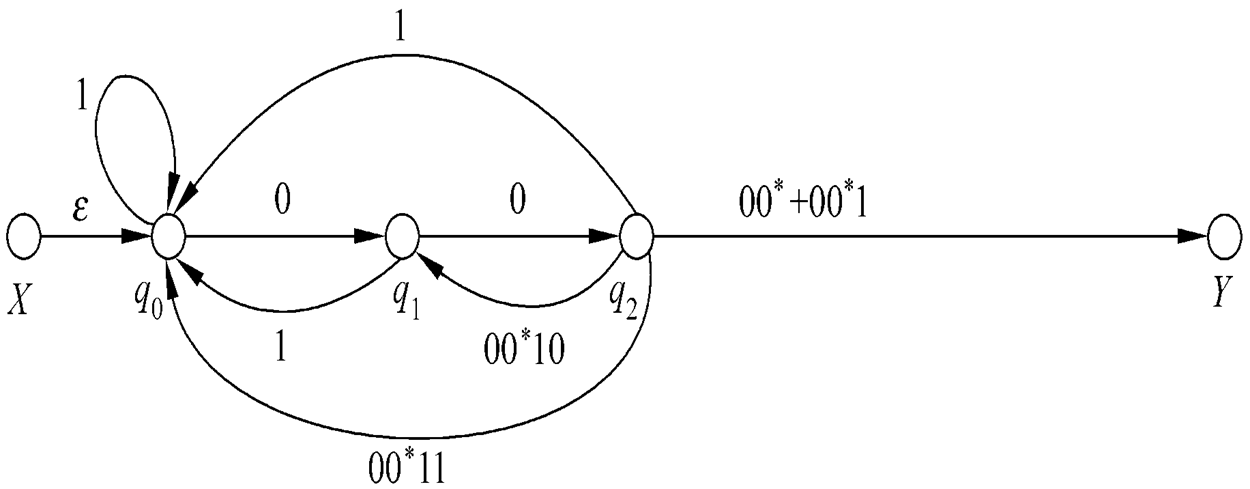
\includegraphics[scale=.45]{ex4-4-4}
	    	\caption{合并后的$DFA$}
	    	\label{fig:ex4-4-4}       % Give a unique label
	    \end{figure}
        \item 去掉状态$q_0$,得到图\ref{fig:ex4-4-5}。
        \begin{figure}[htbp]
        	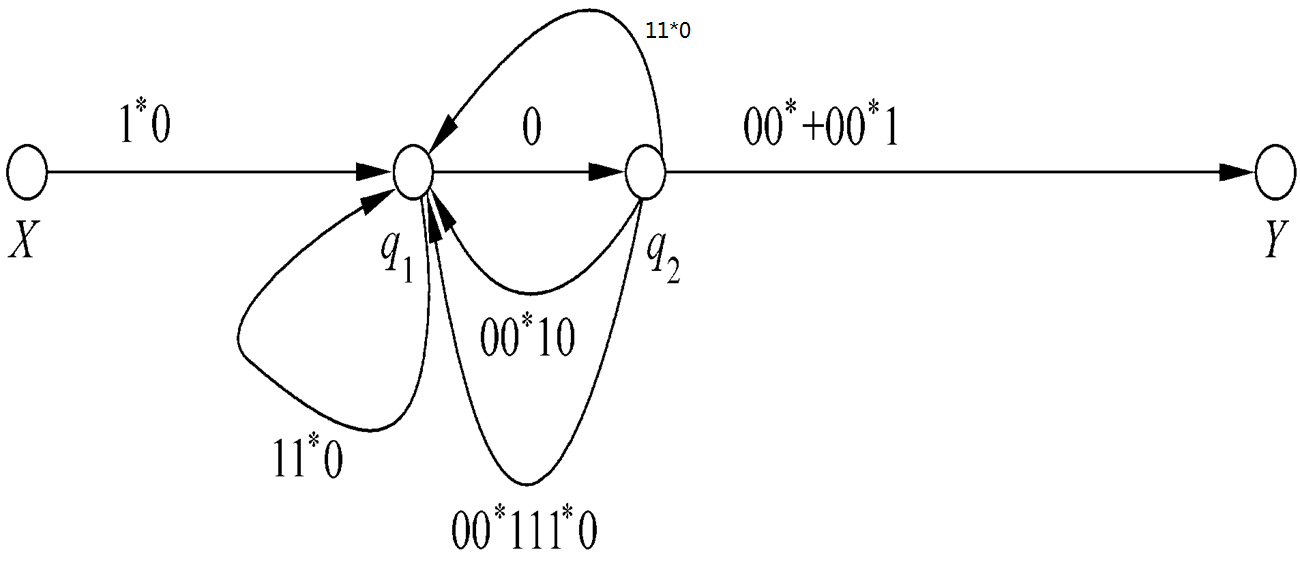
\includegraphics[scale=.3]{ex4-4-5}
        	\caption{去掉状态$q_0$后的$DFA$}
        	\label{fig:ex4-4-5}       % Give a unique label
        \end{figure}
        \item 并弧,得到图\ref{fig:ex4-4-6}。
        \begin{figure}[htbp]
        	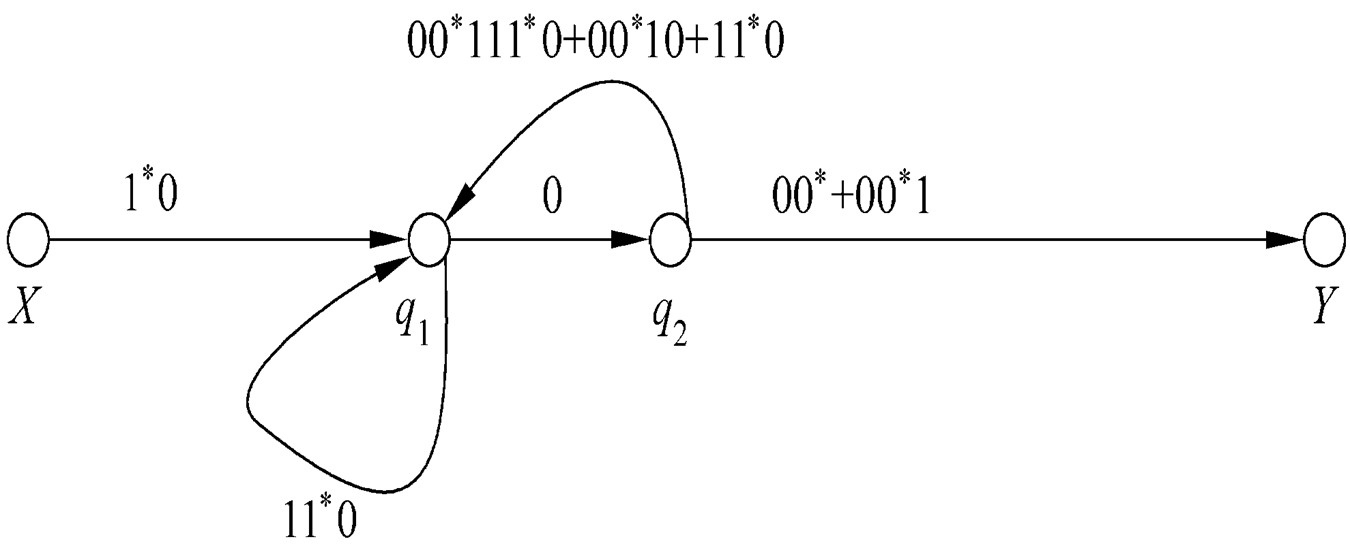
\includegraphics[scale=.45]{ex4-4-6}
        	\caption{并弧后的$DFA$}
        	\label{fig:ex4-4-6}       % Give a unique label
        \end{figure}
        \item 去掉状态$q_1$,得到图\ref{fig:ex4-4-7}。
        \begin{figure}[htbp]
        	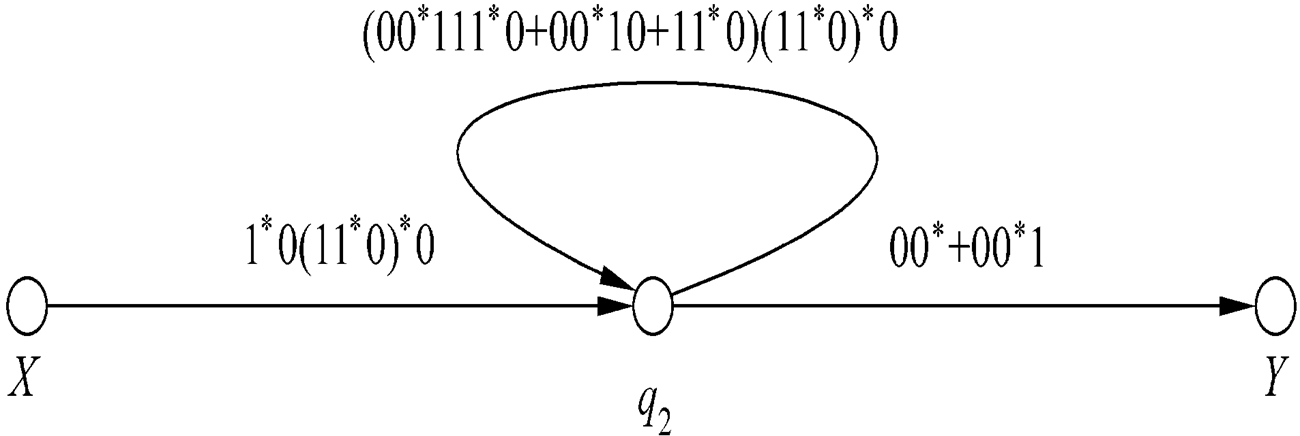
\includegraphics[scale=.45]{ex4-4-7}
        	\caption{去掉状态$q_1$后的$DFA$}
        	\label{fig:ex4-4-7}       % Give a unique label
        \end{figure}\item 去掉状态$q_1$
        \item 去掉状态$q_2$,得到图\ref{fig:ex4-4-8}。
	    \begin{figure}[htbp]
	    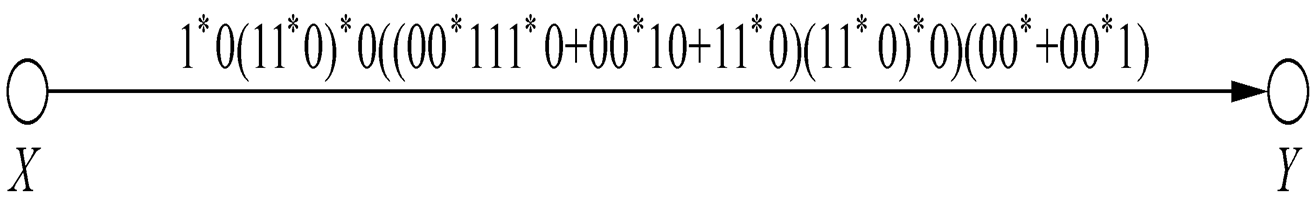
\includegraphics[scale=.45]{ex4-4-8}
	    \caption{去掉状态$q_2$后的$DFA$}
	    \label{fig:ex4-4-8}       % Give a unique label
		\end{figure}
	\end{enumerate}

得到以下正则表达式,就是所求。
$$1^\ast 0(11^\ast 0)^\ast 0((00^\ast 111^\ast 0+00^\ast 10+11^\ast 0)(11^\ast 0)^\ast 0)(00^\ast+00^\ast 1)$$ 
\end{example}

\begin{note}
	以下几点需要注意:
	\begin{enumerate}
		\item 如果去状态的顺序不一样,则得到的$RE$可能在形式是不一样,但它们都是等价的。 
		\item 当$DFA$的终止状态都是不可达的时候,状态转移图中\emph{必不存在}从开始状态到终止状态的路。此时,相应的$RE$为$\emptyset$。
		\item 不计算自身到自身的弧,如果状态$q$的入度为$n$,出度为$m$,则将状态$q$及其相关的弧去掉之后,需要添加$n\times m$条新弧。 
		\item 对操作的步数施归纳,可以证明它的正确性。	
	\end{enumerate}
\end{note}

\begin{corollary}
	正则表达式与$FA$、正则文法等价,是正则语言的表示模型。
\end{corollary}

\section{正则语言等价模型的总结}
到此,一共给出了正则语言的5种等价描述模型:正则文法(RG),确定的有穷状态自动机(DFA),不确定的有穷状态自动机(NFA),带空移动的有穷状态自动机($\epsilon -NFA$),正则表达式(RE)。他们之间的等价转换如图(\ref{fig:model_ev})。
\begin{figure}[htbp]
	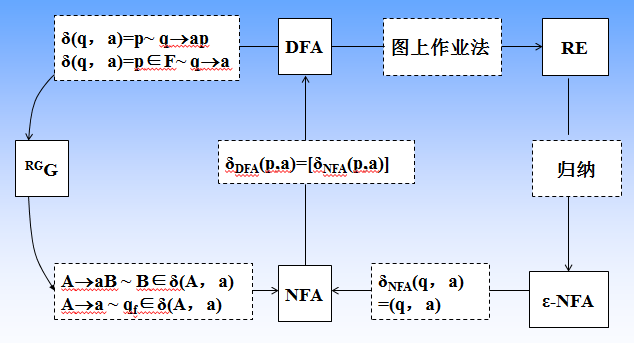
\includegraphics[scale=.6]{model_ev}
	\caption{正则语言5中等价模型的转换}
	\label{fig:model_ev}       % Give a unique label
\end{figure}

\paragraph{小结}
本章讨论了RL及其与FA的等价性。
\begin{enumerate}
	\item 字母表$\Sigma$上的$RE$用来表示$\Sigma$上的$RL$。$\emptyset,\epsilon,a\in\Sigma$是$\Sigma$上的最基本的$RE$,它们分别表示语言$\emptyset,\{\epsilon\},\{a\}$,以此为基础,如果$r$和$s$分别是$\Sigma$上的表示语言$R$和$S$的$RE$,则$r+s,rs,r^\ast$分别是$\Sigma$上的表示语言$R\cup S,RS,R^\ast$的$RE$。如果$L(r)=L(s)$,则称$r$与$s$等价。  
	\item $RE$对乘、加满足结合律;乘对加满足左、右分配律;加满足交换率和幂等率;$\emptyset$是加运算的零元素;$\epsilon$是乘运算的单位元;$\emptyset$是乘运算的零元素。
	\item $RE$是$RL$的一种描述。容易根据$RE$构造出与它等价的$FA$。反过来,可以用图上作业法构造出与给定的$DFA$等价的$RE$。
	\item $RL$的5种等价描述模型转换图。  
\end{enumerate}

\section{Exercise and Solution}
\begin{exercise}
	写出下列语言的正则表达式。
	\begin{enumerate}
		\item ${0,1}^+$。
		\item $\{x|x\in \{0,1\}^\ast \text{且$x$中不含形如$00$的子串}\}$。
	\end{enumerate}	
\end{exercise}

\begin{solution}
	\hfill
	\begin{enumerate}
	\item ${0,1}^+$\\
		  $r=(0+1)(0+1)^\ast$
	\item $\{x|x\in \{0,1\}^\ast \text{且$x$中不含形如$00$的子串}\}$
		\begin{enumerate}
			\item 分析语言,直接构造正则表达式。\\
			$r_1=(1+01)^\ast=\{x|x\text{无连续的0,但以1结尾;当以0开头时,长度不小于2}\}$ \\
			$r_2=(1+10)^\ast=\{x|x\text{无连续的0,以1开头,但以0或者以1结尾;当以0结尾时,长度不小于2}\}$ \\
			$r_3=(1+01)^\ast 0=\{x|x\text{无连续的0,以0结尾;长度至少为1}\}$ \\	
			$r_4= 0 =\{x|x\text{无连续的0,以0开头和结尾;长度为1}\}$ \\
			$\because r_4\subseteq r_3 \\ \therefore r_3 = r_3+r_4$\\
			$r= r_1+r_2+r_3+r_4 = r_1+r_2+r_3$\\		
			$r=(1+01)^\ast + (1+10)^\ast + (1+01)^\ast 0 =(1+10)^\ast + (1+01)^\ast(\epsilon+0)$\\
			\\
			另一种思路是根据$(1+01)^\ast$和$(1+10)^\ast$直接补充所缺部分。\\
			用$0(1+10)^\ast$补上以0开头的满足要求的字符串:\\
			$(1+10)^\ast + 0(1+10)^\ast=(\epsilon + 0)(1+10)^\ast$\\
			或者用$(1+01)^\ast 0$补上以0结尾的满足要求的字符串:\\
			$(1+01)^\ast + (1+01)^\ast 0=(1+01)^\ast(0+\epsilon)$
			\item 图上作业法。\\
			\begin{tabular}{|c|c|}
				\hline 
				\begin{tikzpicture}[>=latex, shorten >=1pt,node distance=0.75in, on grid, auto]
					\node[state,initial,accepting] (q0) {$q_0$};
					\node[state,accepting](q1) [right=of q0] {$q_1$};
					\node[state](dump) [right=of q1] {$d$};
					\path[->]
					(q0) edge [loop above] node {$1$} (q0) 
					(q0) edge [bend left] node {$0$} (q1)
					(q1) edge [bend left] node {$1$} (q0)
					(q1) edge [loop above] node {$1$} (q1) 
					(q1) edge node {$0$} (dump)
					(dump) edge [loop above] node {$0,1$} (dump);
				\end{tikzpicture} & 
				\begin{tikzpicture}[>=latex, shorten >=1pt,node distance=0.75in, on grid, auto]
					\node[state,initial,accepting] (q0) {$q_0$};
					\node[state,accepting](q1) [right=of q0] {$q_1$};
					\node[state,accepting] (q2) [below=of q0] {$q_2$};
					\node[state](dump) [right=of q2] {$d$};
					\path[->]
					(q1) edge [loop above] node {$1$} (q1) 
					(q0) edge [loop above] node {$1$} (q0)
					(q0) edge [bend left] node {$1$} (q1)
					(q1) edge [bend left] node {$0$} (q0)
					(q0) edge node {$0$} (q2)
					(q2) edge [loop below] node {$1$} (q2)
					(q2) edge node {$0$} (dump)
					(dump) edge [loop below] node {$0,1$} (dump);
				\end{tikzpicture} \\
				%\hline 
				(a) NFA: $1^n+(01)^n + 0$ & (b) NFA: $1^n+(10)^n+0$ \\ 
				\hline 
				\begin{tikzpicture}[>=latex, shorten >=1pt,node distance=0.75in, on grid, auto]
				\node[state,initial,accepting] (q0) {$q_0$};
				\node[state,accepting](q1) [right=of q0] {$q_1$};
				\node[state](dump) [right=of q1] {$d$};
				\path[->]
				(q0) edge [loop above] node {$1$} (q0) 
				(q0) edge [bend left] node {$0$} (q1)
				(q1) edge [bend left] node {$1$} (q0)
				(q1) edge node {$0$} (dump)
				(dump) edge [loop above] node {$0,1$} (dump);
				\end{tikzpicture} & 
				\begin{tikzpicture}[>=latex, shorten >=1pt,node distance=0.75in, on grid, auto]
				\node[state,initial,accepting] (q0) {$q_0$};
				\node[state,accepting](q1) [right=of q0] {$q_1$};
				\node[state,accepting] (q2) [below=of q0] {$q_2$};
				\node[state](dump) [right=of q2] {$d$};
				\path[->]
				(q0) edge [loop above] node {$1$} (q0)
				(q0) edge [bend left] node {$1$} (q1)
				(q1) edge [bend left] node {$0$} (q0)
				(q0) edge node {$0$} (q2)
				(q2) edge [loop below] node {$1$} (q2)
				(q2) edge node {$0$} (dump)
				(dump) edge [loop below] node {$0,1$} (dump);
				\end{tikzpicture} \\
				%\hline 
				(c) DFA: $1^n+(01)^n + 0$ & (d) DFA: $1^n+(10)^n+0$ \\ 
				\hline
				\multicolumn{2}{|c|}
				{
					\begin{tikzpicture}[>=latex, shorten >=1pt,node distance=0.75in, on grid, auto]
					\node[state,initial] (q0) {$q_0$};
					\node[state,accepting](q1) [above right=of q0] {$q_1$};
					\node[state,accepting] (q2) [below=of q1] {$q_2$};
					\node[state](dump) [right=of q2] {$d$};
					\path[->]
					(q0) edge node {$1$} (q1)
					(q0) edge node {$0$} (q2)
					(q1) edge [loop above] node {$1$} (q1)
					(q1) edge [swap] node {$0$} (q2)
					(q2) edge [bend right,swap] node {$1$} (q1)
					(q2) edge node {$0$} (dump)
					(dump) edge [loop above] node {0,1} (dump) ;
					\end{tikzpicture} 
				}\\
				%\hline
				\multicolumn{2}{|l|}{构造$\{x|x\in\{0,1\}^+ \text{且$x$中不含形如$00$的子串}\}$语言的$DFA$.}\\ 
				\multicolumn{2}{|l|}{构造要点是,自动机启动并读入一个字符后,就将"精力"集中在考察是否出现$00$子串上,}\\
				\multicolumn{2}{|l|}{一旦发现子串$00$,就进入陷阱状态。}\\
				\hline
			\end{tabular} 
		\end{enumerate}
	\end{enumerate}
\end{solution}

\begin{exercise}
	构造下列正则表达式的等价$FA$。
	$$((0+1)(0+1))^\ast+((0+1)(0+1(0+1))^\ast$$
\end{exercise}

\begin{solution}
	\hfill
	\begin{enumerate}
		\item $(0+1)(0+1))^\ast+((0+1)(0+1(0+1))^\ast$的等价$FA$见图(\ref{fig:0101FA})。
		\item $(0+1)(0+1))^\ast+((0+1)(0+1(0+1))^\ast$的\emph{不等价}$FA$见图(\ref{fig:0101-1FA})。
		\item $(0+1)(0+1))^\ast+((0+1)(0+1(0+1))^\ast$的\emph{不等价}$FA$见图(\ref{fig:0101-2FA})。
		\item $(0+1)(0+1))^\ast+((0+1)(0+1(0+1))^\ast$的\emph{不等价}$FA$见图(\ref{fig:0101-3FA})。
	\end{enumerate}
	\begin{figure}[htbp]
		\centering
		\begin{tikzpicture}[>=latex, shorten >=1pt,node distance=0.75in, on grid, auto]
		\node[state,initial,accepting] (q0) {$q_0$};
		\node[state](q1) [right=of q0] {$q_1$};
		\node[state](q2) [right=of q1] {$q_2$};
		\node[state,accepting](q3) [right=of q2] {$q_3$};
		\node[state] (q4) [below right=of q2] {$q_4$};
		\node[state,accepting](q5) [below=of q1] {$q_5$};
		\node[state] (q6) [left=of q5] {$q_6$};
		\path[->]
		(q0) edge node {$0,1$} (q1)
		(q1) edge node {$0,1$} (q2)
		(q2) edge node {$0,1$} (q3)
		(q3) edge node {$0,1$} (q4)
		(q4) edge node {$0,1$} (q2)
		(q1) edge node {$0,1$} (q5)
		(q5) edge [bend right,swap] node {$0,1$} (q6)	
		(q6) edge [bend right,swap] node {$0,1$} (q5);
		\end{tikzpicture} 
		\caption{$((0+1)(0+1))^\ast+((0+1)(0+1(0+1))^\ast$的等价$FA$}
		\label{fig:0101FA}
	\end{figure}
	\begin{figure}[htbp]
		\begin{tikzpicture}[>=latex, shorten >=1pt,node distance=0.75in, on grid, auto]
		\node[state,initial,accepting] (q0) {$q_0$};
		\node[state](q1) [right=of q0] {$q_1$};
		\node[state](q2) [right=of q1] {$q_2$};
		\node[state,accepting](q3) [right=of q2] {$q_3$};
		\path[->]
		(q0) edge node {$0,1$} (q1)
		(q1) edge node {$0,1$} (q2)
		(q2) edge node {$0,1$} (q3)
		(q1) edge [bend left] node {$0,1$} (q0)	
		(q3) edge [bend left] node {$0,1$} (q1);
		\end{tikzpicture} 
		\caption{$((0+1)(0+1))^\ast+((0+1)(0+1(0+1))^\ast$的\emph{不等价}$FA$}
		\label{fig:0101-1FA}
	\end{figure}
	\begin{figure}[htbp]
		\begin{tikzpicture}[>=latex, shorten >=1pt,node distance=0.75in, on grid, auto]
		\node[state,initial,accepting] (q0) {$q_0$};
		\node[state](q1) [right=of q0] {$q_1$};
		\node[state](q2) [right=of q1] {$q_2$};
		\path[->]
		(q0) edge node {$0,1$} (q1)
		(q1) edge node {$0,1$} (q2)
		(q2) edge [bend right,swap] node {$0,1$} (q0)	
		(q1) edge [bend left] node {$0,1$} (q0);
		\end{tikzpicture} 
		\caption{$((0+1)(0+1))^\ast+((0+1)(0+1(0+1))^\ast$的\emph{不等价}$FA$}
		\label{fig:0101-2FA}
	\end{figure}
	\begin{figure}[htbp]
		\centering
		\begin{tikzpicture}[>=latex, shorten >=1pt,node distance=0.75in, on grid, auto]
		\node[state,initial,accepting] (q0) {$q_0$};
		\node[state](q1) [above right=of q0] {$q_1$};
		\node[state](q2) [right=of q1] {$q_2$};
		\node[state](q3) [below right=of q0] {$q_3$};
		\path[->]
		(q0) edge node {$0,1$} (q1)
		(q1) edge node {$0,1$} (q2)
		(q2) edge node {$0,1$} (q0)
		(q0) edge [bend left] node {$0,1$} (q3)	
		(q3) edge [bend left] node {$0,1$} (q0);
		\end{tikzpicture} 
		\caption{$((0+1)(0+1))^\ast+((0+1)(0+1(0+1))^\ast$的\emph{不等价}$FA$}
		\label{fig:0101-3FA}
	\end{figure}

\end{solution}
	

%%%%%%%%%%%%%%%%%%%%%%%%%%%%%%%%%%%%%%%%%%%%%%%%

\section{正则代换(regular substitution)}

设$\Sigma,\Delta$是两个字母表,映射
$$f:\Sigma \to 2^{\Delta^{\ast}}$$
被称为是从$\Sigma$到$\Delta$的
\textbf{代换}。如果对于$\forall a\in \Sigma,f(a)$是$\Delta$上的$RL$,则称\textbf{$f$为正则代换}。

\begin{itemize}
	\item 现将$f$的定义域扩展到$\Sigma^{\ast}$上:
	\begin{enumerate}
		\item $f(\epsilon) =\{\epsilon\}$
		\item $f(xa)=f(x)f(a)$
	\end{enumerate}
	\item 再将$f$的定义域扩展到$2^{\Delta^{\ast}}$\\
	对于$\forall L\subseteq \Sigma{\ast}$\\
	$f(L) = \bigcup\limits_{x\in L} f(x)$
	\item $f$是正则代换,则
	\begin{enumerate}
		\item $f(\emptyset)=\emptyset$
		\item $f(\epsilon)=\epsilon$
		\item 对于$\forall a\in \Sigma,f(a)$是$\Delta$上的$RE$
		\item 如果$r,s$是$\Sigma$上的$RE$,则\\
		$f(r+s)=f(r)+f(s)$\\
		$f(rs)=f(r)f(s)$\\
		$f(r^{\ast}={f(r)}^{\ast}$\\
		是$\Delta$上的$RE$
	\end{enumerate}
\end{itemize}

\begin{example}
	设$\Sigma={0,1},\Delta={a,b},f(0)=a,f(1)=b^{\ast}$, 则
	\begin{align*}
	f(010) &= f(0)f(1)f(0)=ab^{\ast}a\\
	f({11,00})&=f(11)\cup f(00) \\
	&=f(1)f(1)\cup f(0)f(0)\\
	&=b^{\ast}b^{\ast}+aa = b^{\ast}+aa \\
	f(L(0^{\ast}(0+1)1^{\ast})) &= L(a^{\ast}(a+b^{\ast}){(b^{\ast})}^{\ast})\\
	&= L(a^{\ast}(a+b^{\ast})b^{\ast})\\
	&= L(a^{\ast}ab^{\ast} + a^{\ast}b^{\ast}b^{\ast})\\
	&= L(a^{\ast}b^{\ast})
	\end{align*}
\end{example}

\begin{theorem}
	设$L$是$\Sigma$上的一个$RL$
	$$f:\Sigma \to 2^{\Delta^{\ast}}$$
	是正则代换,则$f(L)$也是$RL$. \hfill$\square$ 
\end{theorem}
\begin{proof}
	描述工具$RE$
	
	对$r$中运算符的个数$n$施以归纳,证明$f(r)$是表示$f(L)$的$RE$.
	\begin{itemize}
		\item 当$n=0$时, 结论成立。
		\item 当$n\le k$时,定理成立,即当$r$中运算符的个数不大于$k$时:$f(L(r)) = L(f(r))$。
		\item 当$n=k+1$时,
		\begin{enumerate}
			\item $r=r_1 + r_2$
			\begin{align*}
			f(L) &= f(L(r)) \\
			&=f(L(r_1 + r_2))\\
			&=f(L(r_1)\cup L(r_2))  &\qquad  \text{$RE$的定义} \\
			&=f(L(r_1))\cup f(L(r_2)) &\qquad \text{正则代换的定义} \\
			&=L(f(r_1))\cup L(f(r_2)) &\qquad \text{归纳假设} \\
			&=L(f(r_1)+f(r_2)) &\qquad RE\text{的定义} \\
			&=L(f(r_1+r_2)) &\qquad RE\text{的正则代换的定义} \\
			&=L(f(r))
			\end{align*}
			
			\item $r=r_1r_2$
			\begin{align*}
			f(L) &=f(L(r)) \\
			&=f(L(r_1r_2))\\
			&=f(L(r_1)L(r2)) &\qquad \text{$RE$的定义}\\
			&=f(L(r_1))f(L(r_2)) &\qquad \text{正则代换的定义}\\
			&=L(f(r_1))L(f(r_2)) &\qquad \text{归纳假设} \\
			&=L(f(r_1)f(r_2)) &\qquad \text{$RE$的定义}\\
			&=L(f(r_1r_2)) &\qquad \text{$RE$的正则代换的定义}\\
			&=L(f(r_1r_2))
			\end{align*}
			
			\item $r={r_1}^{\ast}$
			\begin{align*}
			f(L) &=f(L(r)) \\
			&=f(L({r_1}^{\ast}))\\
			&=f(L({r_1})^{\ast}) &\qquad \text{$RE$的定义}\\
			&={(f(L({r_1})))}^{\ast} &\qquad \text{正则代换的定义}\\
			&={(L(f(r_1)))}^{\ast} &\qquad \text{归纳假设} \\
			&=L(f(r_1)^{\ast}) &\qquad \text{$RE$的定义}\\
			&=L(f({r_1}^{\ast})) &\qquad \text{$RE$的正则代换的定义}\\
			&=L(f(r))
			\end{align*}
		\end{enumerate}
	\end{itemize}  \hfill$\square$ 
\end{proof}
